\documentclass[aspectratio=169]{beamer}
\usefonttheme[onlymath]{serif}

\usepackage[bahasa]{babel}
\usepackage[utf8]{inputenc}
\usepackage[mode=buildnew]{standalone}
\usepackage{algpseudocode}
\usepackage{algorithm}

\usepackage[style=apa]{biblatex}
\usepackage{mathtools}
\usepackage{blindtext}
\usepackage{multicol}
\renewcommand*{\nameyeardelim}{\addcomma\addspace}
\addbibresource{references.bib}

\graphicspath{{resources/}}   % letak direktori penyimpanan gambar

\title[Modifikasi Adam]{Pengembangan dan Implementasi Modifikasi Pengoptimasi Adam pada Lingkungan Terdistribusi}
\author[]{
  Fransiskus Febryan Suryawan\\
  13519124
}
\institute{Institut Teknologi Bandung}
\date{}

\usetheme{venti}

\begin{document}

\clearpage
\pagestyle{empty}

\begin{center}
    \smallskip

    \Large \bfseries \MakeUppercase{\thetitle}
    \vfill

    \Large Laporan Tugas Akhir
    \vfill

    \large Disusun sebagai syarat kelulusan tingkat sarjana
    \vfill

    \large Oleh

    \Large \theauthor

    \vfill
    \begin{figure}[h]
        \centering
        
\includegraphics[width=0.15\textwidth]{cover-ganesha.jpg}
    \end{figure}
    \vfill

    \large
    \uppercase{
        Program Studi Teknik Informatika \\
        Sekolah Teknik Elektro \& Informatika \\
        Institut Teknologi Bandung
    }

    Desember 2022

\end{center}

\clearpage


\section*{Outline}
\begin{frame}{Outline}
  \begin{center}
    \begin{multicols}{2}
      \tableofcontents
    \end{multicols}
  \end{center}
\end{frame}

\section{Pendahuluan}
\subsection{Latar Belakang}
\begin{frame}{Deep Learning}
  \begin{center}
    \includestandalone[height=6em]{figures/dnn}
  \end{center}
  \begin{itemize}
    \item Deep Learning banyak digunakan dalam banyak domain
    \item Sebuah model deep neural network memiliki parameter yang dapat dipelajari
    \item Pembelajaran pada Deep Learning banyak menggunakan teknik \textit{backpropagation}
    \item Arah perkembangan model Deep Learning umumnya adalah memperbanyak parameter untuk mendapat hasil yang lebih baik
  \end{itemize}
\end{frame}

\begin{frame}{\textit{Backpropagation}}
  \begin{itemize}
    \item Digunakan untuk meminimasi \textit{fungsi objektif} $J$
    \item Fungsi objektif $J$ didapatkan dengan membandingkan \textit{output layer} dengan label sebenarnya
    \item Gradien dari fungsi objektif digunakan untuk memperbarui parameter-parameter dari model deep neural network
    \item Gradien untuk layer ke-$l-1$: $$\frac{\partial J}{\partial h^{(l-1)}} = \frac{\partial h^{(l)}}{\partial h^{(l-1)}} \frac{\partial J}{\partial h^{(l)}}$$ dimana J merupakan fungsi objektif yang dipilih
    \item Perhitungan gradien pada layer terakhir dilakukan dengan menurunkan fungsi objektif terhadap \textit{output} layer terakhir
  \end{itemize}
\end{frame}

\begin{frame}{Pengoptimasi Deep Learning}
  \begin{itemize}
    \item Terdapat pengoptimasi untuk backpropagation
          \begin{itemize}
            \item Algoritma yang digunakan untuk mengoptimasi parameter berdasarkan gradien yang didapat pada backpropagation
            \item Menyelesaikan tantangan pada gradient descent
            \item Mempercepat konvergensi model
          \end{itemize}
    \item Pengoptimasi untuk pembelajaran: SGD, \textbf{Adam}, RMSProp, ...
  \end{itemize}
\end{frame}

\begin{frame}{Pengoptimasi Adam}
  \begin{enumerate}
    \item Pengoptimasi digunakan untuk mempelajari parameter pada model
    \item Adam \parencite{ADAMKingma} menggunakan \textit{learning rate} adaptif untuk setiap parameter
    \item Adam menggunakan estimasi momen orde pertama dan kedua untuk membantu pembelajaran
    \item Terdapat modifikasi Adam untuk pembelajaran model Deep Learning Terdistribusi
          \begin{itemize}
            \item CADA: Communication Adaptive Distributed Adam - pengurangan komunikasi \parencite{Chen2021CADA}
            \item Efficient-Adam: kompresi bobot menggunakan kuantisasi \parencite{Chen2022Efficient}
          \end{itemize}
    \item Belum ada modifikasi Adam yang mengurangi komunikasi serta melakukan kuantisasi secara bersamaan
  \end{enumerate}
\end{frame}

\begin{frame}{Deep Learning Terdistribusi}
  \begin{itemize}
    \item Model umum yang digunakan dalam distributed Deep Learning: \textbf{Parameter Server}
    \item Beberapa mesin dapat digunakan secara bersamaan untuk mempercepat pembelajaran model Deep Learning
    \item \textit{Bottleneck}: batasan \textit{bandwidth}
    \item Terdapat usaha untuk mengurangi kebutuhan \textit{bandwidth} untuk bertukar parameter selama pembelajaran
          \begin{itemize}
            \item Kompresi: \textit{lossless}, \textit{lossy}
            \item Pengurangan komunikasi
          \end{itemize}
  \end{itemize}
\end{frame}

\subsection{Rumusan Masalah}
\begin{frame}{Tujuan}
  \begin{itemize}
    \item Menggabungkan teknik pada CADA dengan Efficient-Adam
    \item Membandingkan hasil modifikasi yang telah dibuat dengan CADA
    \item Membandingkan hasil modifikasi yang dibuat dengan Efficient-Adam
  \end{itemize}
\end{frame}


\section{Penelitian Terkait}
\subsection{CADA}
\begin{frame}{CADA \parencite{Chen2021CADA}}
  \begin{itemize}
    \item Terdapat teknik \textit{Lazily Aggregated Gradient} \parencite{Chen2018LAG}
          \begin{itemize}
            \item Keefektifannya berkurang seiring berjalannya pembelajaran
          \end{itemize}
    \item Pengurangan komunikasi berdasarkan kriteria tertentu
    \item Memilih \textit{worker} yang akan mengirim pembaruan parameter, dengan pertaksamaan:
          \begin{itemize}
            \item CADA 1
                  \begin{equation*}
                    \| \delta_m^k - \tilde{\delta}_m^{k-\tau_m^k} \|^2 \le \frac{c}{d_{\mathrm{max}}}\sum_{d=1}^{d_{\mathrm{max}}}\| \theta^{k+1-d} - \theta^{k-d} \|^2
                  \end{equation*}
            \item CADA 2
                  \begin{equation*}
                    \| \nabla \ell (\theta^k; \xi_m^k) - \nabla \ell (\theta_m^{k-\tau_m^k}; \xi_m^k) \|^2 \le \frac{c}{d_{\mathrm{max}}} \sum_{d=1}^{d_{\mathrm{max}}} \| \theta^{k+1-d} - \theta^{k-d} \|^2
                  \end{equation*}
          \end{itemize}
    \item Apabila pertaksamaan tidak dipenuhi, maka \textit{worker} akan mengirimkan pembaruan parameter
  \end{itemize}
\end{frame}

\subsection{Efficient-Adam}
\begin{frame}{Efficient-Adam \parencite{Chen2022Efficient}}
  \begin{itemize}
    \item Kuantisasi untuk mengurangi ukuran parameter serta gradien
          \begin{itemize}
            \item Mengakibatkan presisi turun, mungkin terjadi bias
          \end{itemize}
    \item Error-feedback digunakan untuk mengurangi efek bias
  \end{itemize}
\end{frame}


\section{Rancangan Solusi}
\begin{frame}{Rancangan Solusi}
  \begin{itemize}
    \item Mendesain modifikasi Adam yang menggabungkan CADA \parencite{Chen2021CADA} dan Efficient-Adam \parencite{Chen2022Efficient}
          \begin{itemize}
            \item Harapan: Mengurangi kebutuhan \textit{bandwidth} lebih jauh
          \end{itemize}
    \item Menggunakan pustaka \texttt{PyTorch} untuk abstraksi model Parameter Server serta pembangunan model Deep Learning
    \item Menggunakan kode implementasi CADA dari studi sebelumnya\footnote{\url{https://github.com/ChrisYZZ/CADA-master}} sebagai dasar, dengan modifikasi.
    \item Membuat implementasi Efficient-Adam serta gabungan di atas kerangka dari implementasi CADA yang telah dimodifikasi.
    \item Memilih fungsi kuantisasi yakni pemetaan dari float64 ke float16
  \end{itemize}
\end{frame}

\begin{frame}{Rancangan Solusi}
  \begin{itemize}
    \item Menguji implementasi CADA, Efficient-Adam, serta gabungan.
    \item Membandingkan akurasi model, jumlah komunikasi, serta ukuran data yang digunakan untuk komunikasi dalam pengujian
  \end{itemize}
\end{frame}


\section{Implementasi dan Pengujian}
\begin{frame}{Implementasi}
  \begin{itemize}
    \item Parameter Server, untuk menjalankan tugas sebagai parameter server
    \item Trainer, untuk menjalankan tugas sebagai worker
    \item Runner, untuk mengorkestrasi Parameter Server dengan Trainer
  \end{itemize}
\end{frame}

\subsection{Algoritma}
\begin{frame}{Algoritma Parameter Server}
  \begin{algorithm}[H]
    \caption{Algoritma Parameter Server}
    \begin{algorithmic}[1]
      \State \textbf{Parameter:} Fungsi Kuantisasi $\mathcal{Q}_s$
      \State \textbf{Inisialisasi} vektor parameter $\theta_0$, error term $e_1 \gets 0$
      \State Sebarkan $\theta_0$ ke semua \textit{worker}
      \For{$t = 1,2,\dots,T$}
      \State $\hat{\delta_t} \gets \textnormal{rata-rata } \delta_t^{(i)}$ dari setiap \textit{worker}
      \State Sebarkan $\tilde{\delta_t} \gets \mathcal{Q}(\hat{\delta_t} + e_t)$
      \State $e_{t+1} \gets e_{t}$
      \State $\theta_{t+1} \gets \theta_t - \tilde{\delta_t}$
      \EndFor
    \end{algorithmic}
  \end{algorithm}
\end{frame}

\begin{frame}{Algoritma Worker}
  \begin{algorithm}[H]
    \caption{Modifikasi Adam untuk Worker ke-$i$}
    \begin{algorithmic}[1]
      \State \textbf{Parameter:} Fungsi Kuantisasi $\mathcal{Q}_w$, Hyperparameter Adam $\alpha, \beta_1, \beta_2$, konstanta batas $c$, batas maksimum penundaan $D$
      \State $m_0^{(i)} \gets 0, v_0^{(i)} \gets \epsilon, e_1^{(i)} \gets 0, \tau^{(i)} \gets 0$
      \State $\theta^{(i)}_0 \gets \theta_1$ dari server
      \For{$t=1,2,\dots,T$}
      \State $g_t^{(i)} \gets \nabla_\theta f_t(\theta_{t})$
      \State $v_t^{(i)} \gets \theta_t v_{t-1}^{(i)} + (1-\theta_t)[g_t^{(i)}]^2$
      \State $m_t^{(i)} \gets \beta_1 m_{t-1}^{(i)} + (1-\beta_1)g_t^{(i)}$
      \State $\alpha_t \gets \alpha \sqrt{1-\beta_2^t}/(1-\beta_1^t)$
      \State $\delta^{(i)} \gets \alpha_t m_t^{(i)}/\sqrt{v_t^{(i)}}+e_t^{(i)}$
      \State $\theta_t \gets \theta_{t-1} - \delta^{(i)}$
      \algstore{worker}
    \end{algorithmic}
  \end{algorithm}
\end{frame}

\begin{frame}{Algoritma Worker}
  \begin{algorithm}[H]
    \begin{algorithmic}[1]
      \algrestore{worker}
      \State Hitung $\nabla f_t(\theta^{(i)}_{t})$ dan $\nabla f_t(\theta^{(i)}_{t-\tau})$
      \State $\delta^{(i)} \gets \mathcal{Q}_w(\delta^{(i)})$
      \If{Kondisi \ref{cada2cond} tidak terpenuhi atau $\tau \ge D$}
      \State Kirim $\delta^{(i)}$
      \State $\tau \gets 1$
      \Else
      \State $\tau \gets \tau + 1$
      \EndIf
      \State $e_{t+1}^{(i)} \gets \alpha_t \frac{m_t^{(i)}}{\sqrt{v_t^{(i)}}} + e_t^{(i)} - \delta_t^{(i)}$
      \State Terima $\tilde{\delta_t}$ dari server
      \State $\theta_{t} \gets \theta_{t-1} - \tilde{\delta_t}$
      \EndFor
    \end{algorithmic}
  \end{algorithm}
\end{frame}

\begin{frame}{Kondisi Worker}
  \begin{equation}
    \label{cada2cond}
    \|\nabla f_t(\theta_t) - \nabla f_t(\theta_{t-\tau})\|^2 \leq \frac{c}{D} \sum_{d=1}^{D} \|\theta_{t+1-d} - \theta_{t-d}\|^2
  \end{equation}
\end{frame}

\subsection{Lingkungan Pengujian}
\begin{frame}{Lingkungan Pengujian}
  Pengujian dilakukan pada server DGX, menggunakan satu GPU yang dialokasikan. Setiap trainer dan parameter server dijalankan pada GPU yang sama.

  \begin{table}
    \caption{Spesifikasi Server DGX}
    \centering
    \begin{tabular}[ht]{ | c | c | }
      \hline
      \textbf{Parameter} & \textbf{Spesifikasi}                           \\
      \hline
      CPU                & 2x Intel Xeon E5-2698 v3 (16-core, Haswell-EP) \\
      \hline
      RAM                & 512GB DDR4-2133                                \\
      \hline
      GPU                & 8x Tesla V100 32GB VRAM                        \\
      \hline
      Penyimpanan        & 4x1.92 TB SSD                                  \\
      \hline
    \end{tabular}
  \end{table}
\end{frame}

\begin{frame}{Lingkungan Pengujian}
  Versi kakas dan pustaka yang digunakan dalam pengujian
  \begin{table}
    \caption{Versi Perangkat Lunak}\label{softwares}
    \centering
    \begin{tabular}{ | c | c | }
      \hline
      \textbf{Perangkat Lunak} & \textbf{Versi} \\
      \hline
      Python                   & 3              \\
      \hline
      PyTorch                  & 1.13.1+cuda    \\
      \hline
      TorchVision              & 0.14.1+cuda    \\
      \hline
    \end{tabular}
  \end{table}
\end{frame}

\subsection{Skenario Pengujian}
\begin{frame}{Skenario Pengujian}
  Terdapat dua skenario yang akan diuji untuk membandingkan teknik-teknik yang telah disebutkan.
  \begin{itemize}
    \item Pelatihan model sederhana untuk mempelajari dataset Fashion-MNIST \parencite{xiao2017fashion}.
    \item Pelatihan ResNet-20 untuk mempelajari dataset CIFAR10 \parencite{krizhevsky2009cifar}.
  \end{itemize}
\end{frame}

\subsubsection{Fashion-MNIST}
\begin{frame}{Fashion-MNIST}
  \begin{itemize}
    \item Fashion-MNIST \parencite{xiao2017fashion} adalah suatu \textit{dataset} yang berisi 60000 gambar pakaian berukuran 28 $\times$ 28 piksel dari Zalando.

    \item Akan digunakan model sederhana untuk melakukan klasifikasi. Arsitektur model dapat dilihat pada gambar berikut.
  \end{itemize}
  \begin{figure}
    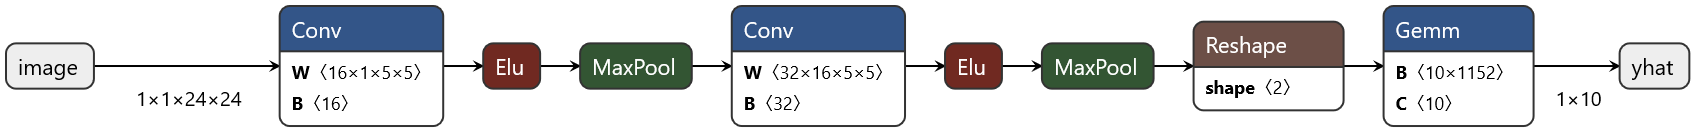
\includegraphics[width=13cm]{fashion_mnist.onnx.png}
    \caption{Model sederhana untuk klasifikasi Fashion-MNIST}\label{modelfashion}
  \end{figure}
\end{frame}

\begin{frame}{Hyperparameter}
  \begin{columns}[b]
    \begin{column}{3.5cm}
      Hyperparameter untuk CADA \\
      \vspace{1cm}
      \begin{tabular}{ | c | c | }
        \hline
        \textbf{Parameter} & \textbf{Nilai} \\
        \hline
        $\alpha$           & 0.00001        \\
        \hline
        $\beta_1$          & 0.9            \\
        \hline
        $\beta_2$          & 0.99           \\
        \hline
        $D$                & 50             \\
        \hline
        $d_{max}$          & 10             \\
        \hline
        $c$                & 400            \\
        \hline
      \end{tabular}
    \end{column}
    \begin{column}{3.5cm}
      Hyperparameter untuk Efficient-Adam \\
      \vspace{1cm}
      \begin{tabular}{ | c | c | }
        \hline
        \textbf{Parameter} & \textbf{Nilai} \\
        \hline
        $\alpha$           & 0.0001         \\
        \hline
        $\beta_1$          & 0.9            \\
        \hline
        $\beta_2$          & 0.999          \\
        \hline
      \end{tabular}
    \end{column}
    \begin{column}{3.5cm}
      Hyperparameter untuk gabungan \\
      \vspace{1cm}
      \begin{tabular}{ | c | c | }
        \hline
        \textbf{Parameter} & \textbf{Nilai} \\
        \hline
        $\alpha$           & 0.0001         \\
        \hline
        $\beta_1$          & 0.9            \\
        \hline
        $\beta_2$          & 0.99           \\
        \hline
        $D$                & 50             \\
        \hline
        $d_{max}$          & 10             \\
        \hline
        $c$                & 400            \\
        \hline
      \end{tabular}
    \end{column}
  \end{columns}
\end{frame}

\subsubsection{CIFAR10}
\begin{frame}{CIFAR10}
  \begin{itemize}
    \item CIFAR10 \parencite{krizhevsky2009cifar} merupakan dataset yang berisi 60.000 gambar berwarna berukuran 32 $\times$ 32 piksel. Seluruh gambar diklasifikasi ke dalam 10 kelas yang berbeda.
    \item Akan digunakan model ResNet-20 \parencite{Idelbayev18a} untuk melakukan klasifikasi terhadap dataset CIFAR10. Model ResNet memiliki \textit{building block} berupa \textit{residual block} yang diilustrasikan pada gambar di bawah.
  \end{itemize}
  \begin{figure}
    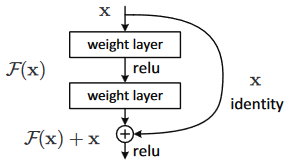
\includegraphics{resblock.png}
    \caption{Blok residu dalam ResNet \parencite{Idelbayev18a}}
  \end{figure}
\end{frame}

\begin{frame}{Hyperparameter}
  \begin{columns}[b]
    \begin{column}{3.5cm}
      Hyperparameter untuk CADA \\
      \vspace{1cm}
      \begin{tabular}{ | c | c | }
        \hline
        \textbf{Parameter} & \textbf{Nilai} \\
        \hline
        $\alpha$           & 0.01           \\
        \hline
        $\beta_1$          & 0.9            \\
        \hline
        $\beta_2$          & 0.99           \\
        \hline
        $D$                & 50             \\
        \hline
        $d_{max}$          & 2              \\
        \hline
        $c$                & 0.12           \\
        \hline
      \end{tabular}
    \end{column}
    \begin{column}{3.5cm}
      Hyperparameter untuk Efficient-Adam \\
      \vspace{1cm}
      \begin{tabular}{ | c | c | }
        \hline
        \textbf{Parameter} & \textbf{Nilai} \\
        \hline
        $\alpha$           & 0.0005         \\
        \hline
        $\beta_1$          & 0.9            \\
        \hline
        $\beta_2$          & 0.999          \\
        \hline
      \end{tabular}
    \end{column}
    \begin{column}{3.5cm}
      Hyperparameter untuk gabungan \\
      \vspace{1cm}
      \begin{tabular}{ | c | c | }
        \hline
        \textbf{Parameter} & \textbf{Nilai} \\
        \hline
        $\alpha$           & 0.0005         \\
        \hline
        $\beta_1$          & 0.9            \\
        \hline
        $\beta_2$          & 0.999          \\
        \hline
        $D$                & 50             \\
        \hline
        $d_{max}$          & 2              \\
        \hline
        $c$                & 0.12           \\
        \hline
      \end{tabular}
    \end{column}
  \end{columns}
\end{frame}

\subsection{Hasil Pengujian}
\subsubsection{Fashion-MNIST}
\begin{frame}{Hasil Pengujian terhadap Fashion-MNIST}
  \begin{center}
    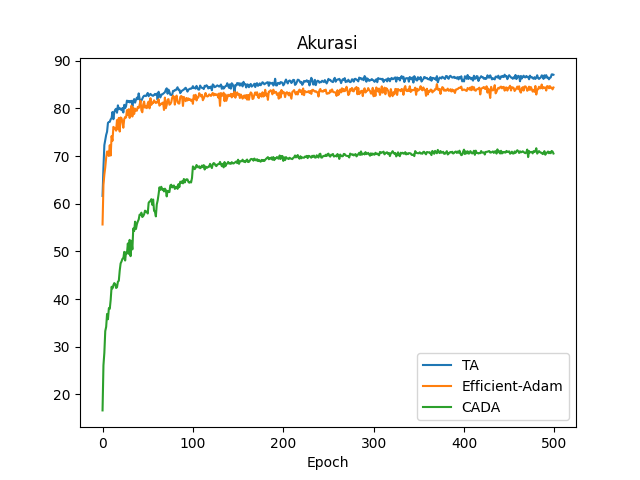
\includegraphics[width=6.5cm]{fashion_acc.png}
  \end{center}
  Akurasi tertinggi didapatkan oleh teknik gabungan, yang berada di sekitar 86\%. Sedangkan akurasi terendah didapatkan oleh CADA, di sekitar 70\%.
\end{frame}

\begin{frame}{Hasil Pengujian terhadap Fashion-MNIST}
  \begin{center}
    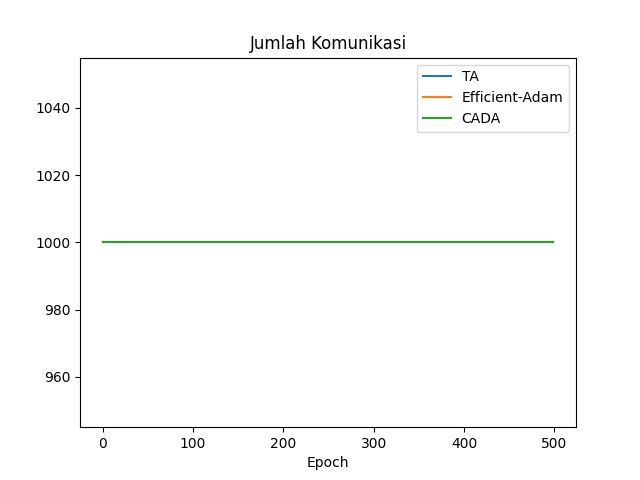
\includegraphics[width=6.5cm]{fashion_comms.png}
    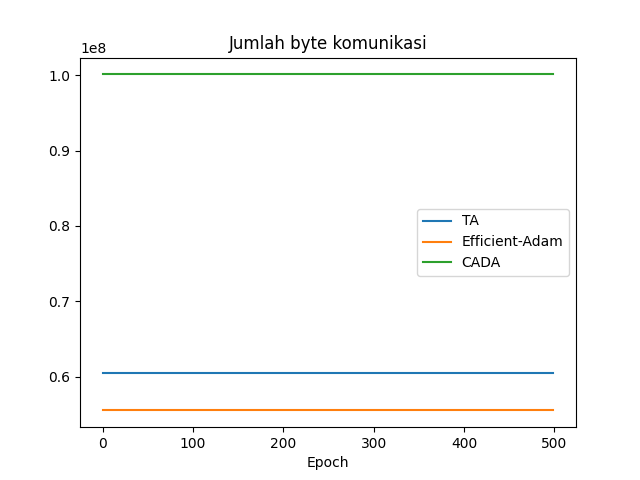
\includegraphics[width=6.5cm]{fashion_bits.png}
  \end{center}
  Jumlah komunikasi sama untuk setiap teknik, namun jumlah byte yang digunakan Efficient-Adam dan teknik gabungan jauh lebih sedikit dibandingkan CADA karena kompresi.
\end{frame}

\subsubsection{CIFAR10}
\begin{frame}{Hasil Pengujian terhadap CIFAR-10}
  \begin{center}
    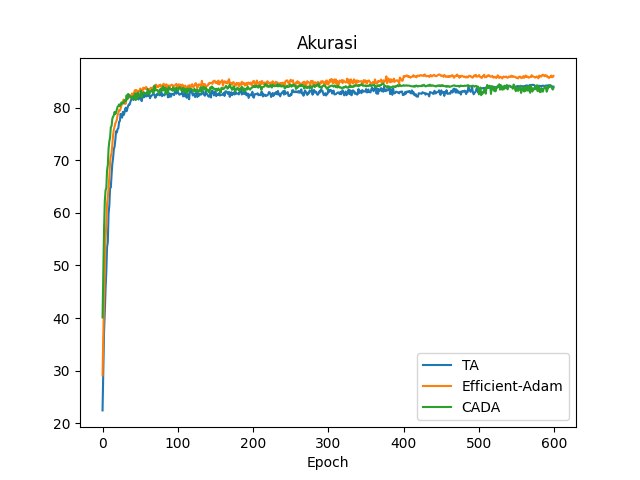
\includegraphics[width=6.5cm]{resnet_acc.png}
  \end{center}
  Akurasi yang didapatkan berada di sekitar 84-86\% untuk setiap teknik, dengan Efficient-Adam memiliki akurasi tertinggi.
\end{frame}

\begin{frame}{Hasil Pengujian terhadap CIFAR-10}
  \begin{center}
    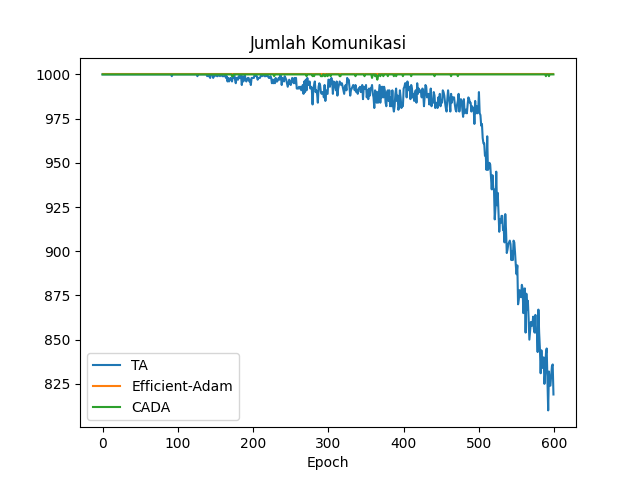
\includegraphics[width=6.5cm]{resnet_comms.png}
    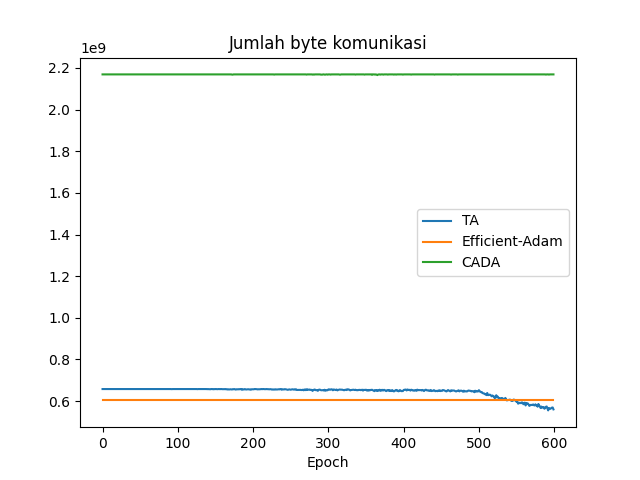
\includegraphics[width=6.5cm]{resnet_bits.png}
  \end{center}
  Jumlah komunikasi dikurangi paling banyak oleh teknik gabungan, dengan CADA mengurangi komunikasi pada beberapa epoch tertentu saja. Jumlah byte yang digunakan paling sedikit oleh Efficient-Adam, namun teknik gabungan mampu mengurangi jumlah byte karena jumlah komunikasi yang berkurang.
\end{frame}

\subsection{Analisis Hasil Pengujian}
\begin{frame}{Analisis Hasil Pengujian}
  \begin{itemize}
    \item Teknik gabungan menggunaka jumlah byte yang lebih sedikit dibanding CADA, namun lebih banyak dibandingkan Efficent-Adam.
    \item Jumlah byte tambahan yang digunakan dalam teknik gabungan adalah komunikasi nilai ambang.
    \item Pengurangan jumlah komunikasi dalam skenario Fashion-MNIST tidak ada, karena jumlah parameter yang lebih sedikit, nilai ambang akan lebih kecil sehingga lebih mudah untuk mencapai nilai tersebut.
    \item Pengurangan jumlah komunikasi dalam skenario CIFAR10 lebih banyak, karena nilai ambang yang lebih besar.
    \item Jumlah komunikasi pada CADA tidak berkurang banyak karena pemilihan \textit{hyperparameter} yang menyebabkan selisih gradien besar.
    \item Pemilihan \textit{hyperparameter} yang berbeda menyebabkan model lebih sulit konvergen ke akurasi yang lebih tinggi.
  \end{itemize}
\end{frame}


\section{Kesimpulan dan Saran}
\subsection{Kesimpulan}
\begin{frame}{Kesimpulan}
  \begin{itemize}
    \item Berhasil menggabungkan teknik Efficient-Adam dengan CADA
    \item Teknik gabungan menggunakan jumlah komunikasi yang lebih sedikit dibandingkan CADA
    \item Teknik gabungan menggunakan jumlah byte lebih banyak dibandingkan Efficient-Adam, namum tetap lebih sedikit dibandnigkan CADA.
  \end{itemize}
\end{frame}

\subsection{Saran}
\begin{frame}{Saran}
  \begin{itemize}
    \item Memilih teknik lain untuk digabungkan
    \item Memilih \textit{domain} lain selain computer vision
    \item Menggunakan \textit{dataset} lain
  \end{itemize}
\end{frame}


\section*{Pertanyaan}
\begin{frame}
  \vfill
  \centering
  \begin{beamercolorbox}[sep=8pt,center]{title}
    \usebeamerfont{title}\insertsectionhead\par
  \end{beamercolorbox}
\end{frame}

\end{document}
